\begin{figure}[H]
\centering
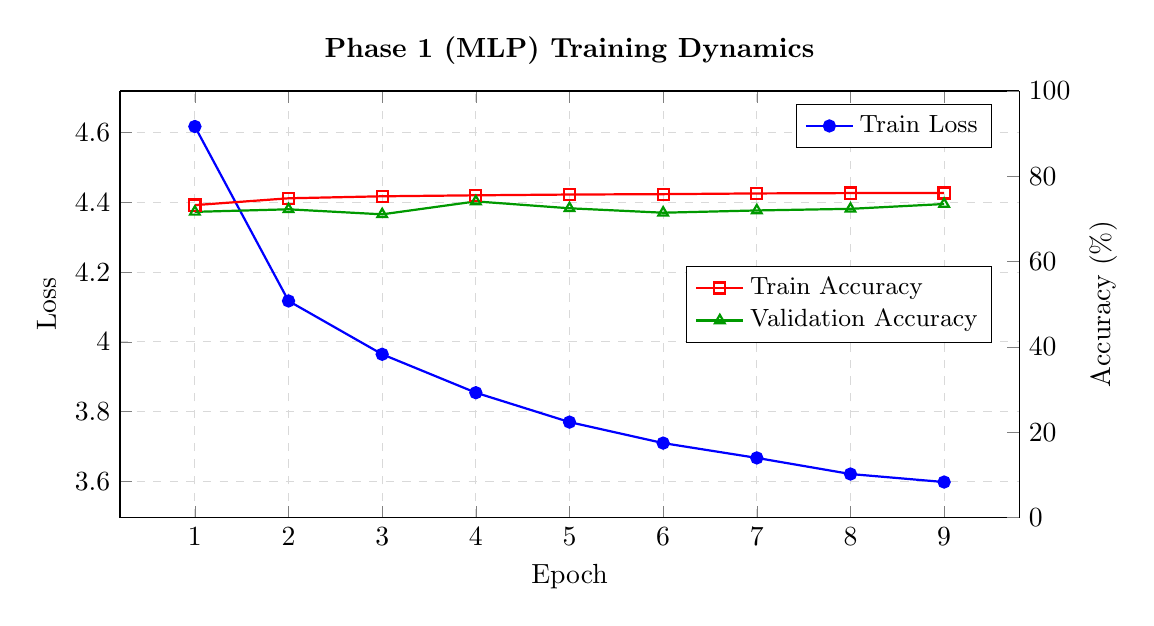
\begin{tikzpicture}
\begin{axis}[
    width=13cm, height=7cm,
    xlabel={Epoch}, ylabel={Loss},
    axis y line*=left,
    grid=major, grid style={dashed,gray!30},
    legend pos=north east, legend cell align=left,
    legend style={font=\small},
    title={\textbf{Phase 1 (MLP) Training Dynamics}},
]
\addplot[blue, thick, mark=*] coordinates {
    (1, 4.6176)
    (2, 4.1173)
    (3, 3.9644)
    (4, 3.8542)
    (5, 3.7699)
    (6, 3.7097)
    (7, 3.6672)
    (8, 3.6210)
    (9, 3.5980)
};
\addlegendentry{Train Loss}
\end{axis}
\begin{axis}[
    width=13cm, height=7cm,
    axis y line*=right, axis x line=none,
    ylabel={Accuracy (\%)},
    ymin=0, ymax=100,
    legend style={at={(0.97,0.50)}, anchor=east, font=\small},
    legend cell align=left,
]
\addplot[red, thick, mark=square] coordinates {
    (1, 73.24)
    (2, 74.84)
    (3, 75.31)
    (4, 75.54)
    (5, 75.72)
    (6, 75.81)
    (7, 75.98)
    (8, 76.06)
    (9, 76.09)
};
\addlegendentry{Train Accuracy}
\addplot[green!60!black, thick, mark=triangle] coordinates {
    (1, 71.66)
    (2, 72.26)
    (3, 71.08)
    (4, 74.11)
    (5, 72.50)
    (6, 71.46)
    (7, 71.99)
    (8, 72.37)
    (9, 73.50)
};
\addlegendentry{Validation Accuracy}
\end{axis}
\end{tikzpicture}
\caption{Phase 1 (MLP) training dynamics over 9 epochs. Best validation accuracy
of 74.11\% at epoch 4. Training accuracy plateaus around 76\%.}
\label{fig:p1_training_dynamics}
\end{figure}
